\documentclass[11pt]{article}

\usepackage[margin=1in]{geometry}
\usepackage[T1]{fontenc}
\usepackage{lmodern}
\usepackage{microtype}
\usepackage{graphicx}
\usepackage{booktabs}
\usepackage{array}
\usepackage{amsmath,amssymb}
\usepackage{enumitem}
\usepackage[dvipsnames]{xcolor}
\usepackage[round,authoryear]{natbib}
\usepackage[colorlinks=true,allcolors=MidnightBlue]{hyperref}
\usepackage[nameinlink,noabbrev]{cleveref}

\setlist{nosep}
\graphicspath{{figures/}}
\hypersetup{
  pdftitle={GAWorld: Building Persistent and Situated LLM Agent Societies},
  pdfauthor={},
  pdfsubject={LLM-based artificial societies and multi-agent social simulation},
  pdfkeywords={LLM agents, multi-agent systems, artificial societies, social simulation}
}

\title{GAWorld: Building Persistent and Situated LLM Agent Societies}
\author{Author Name(s)\\Affiliation(s)\\\texttt{email@example.org}}
\date{2026}

\begin{document}
\maketitle

\begin{abstract}
GAWorld is research infrastructure for constructing persistent, situated, and inspectable societies of
large-language-model agents. It connects agent profiles, state, memory, planning, and reflection to an
urban environment, social relations, economic processes, work, and controlled interventions. This paper
documents the implemented system, its incremental migration toward a composable execution architecture,
its research interfaces, and the scope of its existing experimental artifacts. The current evidence is used
to demonstrate system affordances and limitations rather than to claim prediction of real populations or
policy effects.
\end{abstract}

\section{Introduction}
GAWorld addresses the systems problem of connecting persistent LLM agents to a shared, inspectable social
simulation rather than evaluating isolated conversations or short-lived task episodes.

\section{Design Goals}
The system is organized around persistence, situatedness, composability, controllability, inspectability,
and compatibility with a progressively modularized runtime.

\section{Related Work}
GAWorld intersects research on generative agents, social-agent evaluation, agent-based simulation, and
modular execution architectures while targeting the integration of these concerns in one research system.

\section{Agent Lifecycle}
At each simulation step, an agent combines its profile and state with situated perception and recalled
experience before planning, acting, reflecting, and persisting the resulting trace.

\section{Execution Architecture and Incremental Modularization}
\label{sec:execution-architecture}

GAWorld's runtime combines a connected cognition pipeline with a small kernel
and compatibility-preserving domain paths.  Figure~\ref{fig:system-architecture}
distinguishes stable connections from the incomplete plugin migration.  This
distinction matters scientifically: a mechanism that can be configured or
observed is not necessarily isolated enough to be exchanged without changing
other runtime behavior.

\begin{figure}[t]
  \centering
  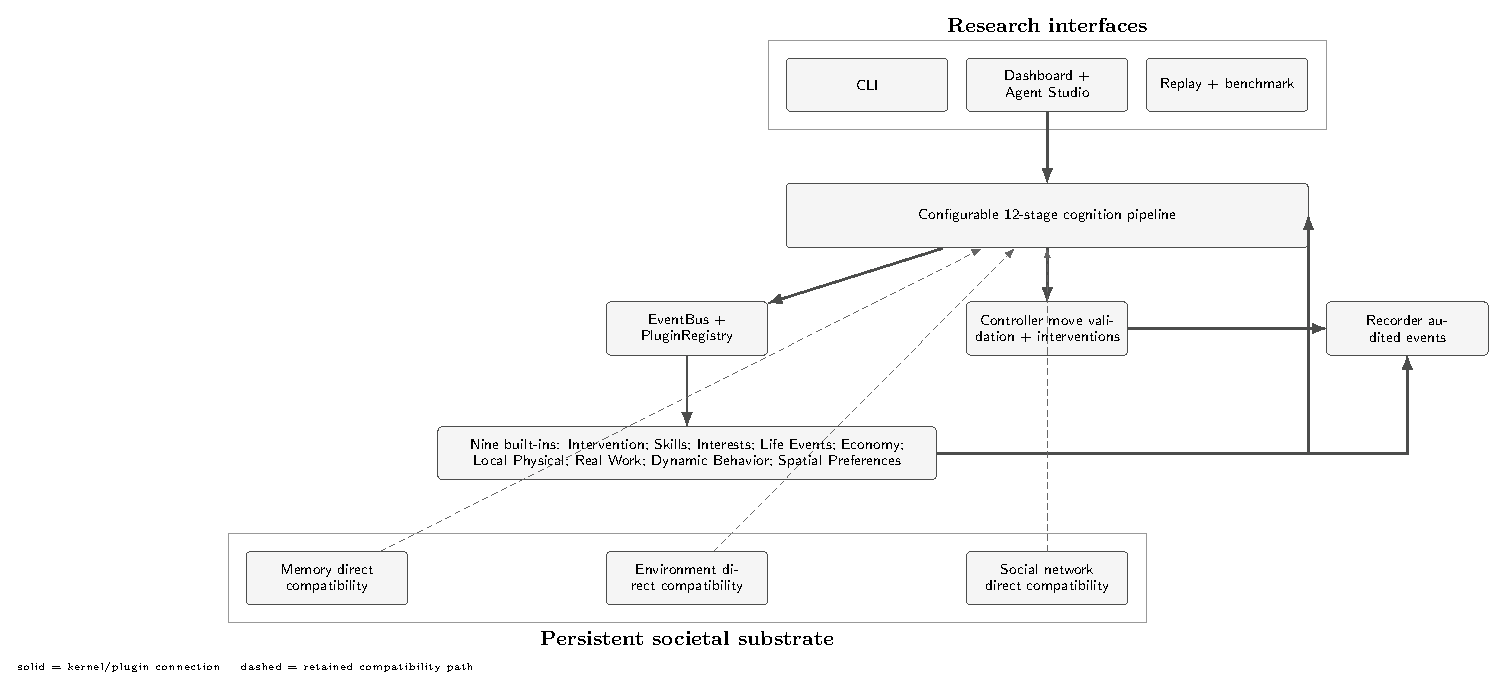
\includegraphics[width=\linewidth]{system_architecture.pdf}
  \caption{Audited execution architecture.  Solid paths denote connected
  implementation surfaces; dashed paths denote a partial or skeleton path.
  The committed built-in plugins are Intervention, Skills, Interests, and Life
  Events.  Memory, world, social, and work logic
  retain direct paths, while economy integration is primarily hook-based.}
  \label{fig:system-architecture}
\end{figure}

\subsection{Kernel services}

\paragraph{Simulation context.}
\texttt{SimContext} is the object shared by stages and plugins.  It holds
configuration, the Clock, EventBus, PluginRegistry, Controller, Recorder,
agents and their identifier index, an LLM callable, a seeded random-number
generator, and an \texttt{extras} escape hatch for objects not yet formalized
by the kernel.  It also provides simulation-level and per-agent plugin state
namespaces.  The bootstrap constructs this context, installs it in every bus
dispatch, attaches the city map through \texttt{extras}, and refreshes the
agent index.  The escape hatch and mutable dictionaries preserve compatibility
but limit enforcement of ownership boundaries.

\paragraph{Clock.}
The Clock stores simulated day, time string, tick index, and optionally the
minutes per tick.  The outer loop is its sole writer: it starts each day and
advances before processing a tick.  Stages, plugins, and Recorder can therefore
share a time coordinate without receiving separate arguments.  The clock
orders simulation events; it does not make a run deterministic, because model
responses, external services, concurrency, and unseeded dependencies may still
vary.

\paragraph{Event bus.}
The EventBus is a priority-ordered superset of the earlier HookBus.  Its
\texttt{emit} operation notifies observers, \texttt{collect} merges
contributions, and \texttt{filter} passes a value through possible rewrites.
It retains the existing configuration-driven hook format and adds the
\texttt{SimContext} to dispatch data.  Handler exceptions are logged and
isolated by default, with optional strict failure.  This policy keeps an
auxiliary observer from terminating a run, but it can yield a degraded run;
logs and active-plugin lists must therefore be retained with results.

\paragraph{Plugin registry.}
The PluginRegistry assembles built-in instances, configuration-named classes,
and installed entry points.  It rejects duplicate or invalid identifiers,
orders setup by declared dependencies, deactivates a plugin whose setup fails
or whose dependency is unavailable, and tears active plugins down in reverse
order.  A plugin may own configuration, \texttt{agent["ext"]} state, and an
output directory.  This is a functional lifecycle boundary, but it is not a
sandbox: third-party code runs in process, entry points are not allowlisted,
and compatibility modules may still mutate common agent state.

\paragraph{Controller.}
The Controller defines two interfaces.  First, a priority-ordered validator
chain can allow, deny, or rewrite a structured \texttt{ActionRequest}; denials
are sent to the Recorder.  Second, named runtime interventions can be
registered and invoked with an audit record.  These interfaces are implemented
and unit-testable, but they remain a skeleton relative to the principal
simulator: selected actions and ordinary intervention mechanisms do not all
flow through the Controller.  We therefore do not treat it as a universal
policy or safety gate.

\paragraph{Recorder.}
The Recorder appends clock-stamped JSON objects to a table-per-file store and
is closed when the simulation exits.  It currently records Controller-mediated
events and is available to extensions.  The main trace, state-history, memory,
environment, and plugin metric paths continue to use their established writers.
The Recorder is thus a basis for future unified replay, not evidence that the
current archive can be replayed from one event log.

\subsection{A concrete plugin migration}

The committed \texttt{InterventionPlugin} illustrates what has actually moved
onto the kernel boundary.  During setup it subscribes to three points.  At
\texttt{agents.built}, it seeds intervention metric keys so initial snapshots
retain a consistent schema.  When enabled, it contributes a recommendation
feed at \texttt{perception.compose}, stores temporary feed data in its
per-agent extension namespace, and updates and persists intervention metrics
at \texttt{on\_agent\_post\_step}.  The plugin delegates domain calculations
to the existing policy implementation; migration changes orchestration and
ownership rather than reimplementing the research mechanism.

Skills, Interests, and Life Events are also committed built-in plugins.  The
\texttt{LifeEventsPlugin}, the fourth built-in and the first event-producer
migration, subscribes to day and tick boundaries, composes environmental event
views, contributes agent-specific event context to perception, and applies
declared state effects.  It delegates queue persistence and domain operations
to the established life-event implementation, so the migration changes
orchestration rather than validating event realism.  Archived runs in this
paper predate that migration and are not attributed to it.  No completed plugin
claim is made for economy, memory, world, social, or work.

\subsection{Migration-state audit}

Table~\ref{tab:migration-state} summarizes the distinction between code
presence and runtime integration.  ``Direct'' denotes calls retained in the
simulation or stage implementation; ``hook-based'' denotes established event
callbacks that need not be registered as kernel plugins.

\begin{table}[t]
\centering
\small
\setlength{\tabcolsep}{4pt}
\begin{tabular}{@{}p{0.14\linewidth}p{0.23\linewidth}p{0.16\linewidth}p{0.19\linewidth}p{0.20\linewidth}@{}}
\toprule
Surface & Current implementation & Integration status & Compatibility path & Research consequence \\
\midrule
Cognition & Configured 12-stage pipeline & Wired & Shared step dictionary and outer-loop work & Stage order and omissions must be reported \\
Event extensions & EventBus with emit, collect, and filter & Wired & Legacy hook signatures/configuration & Observer failure can degrade rather than stop a run \\
Intervention & \texttt{InterventionPlugin} plus policy implementation & Plugin-integrated & Domain logic and specialized metric writer retained & Feed contribution and metrics are inspectable; causal validity is separate \\
Skills and interests & Committed built-in plugins & Plugin-integrated & Existing agent and memory fields remain readable & Lifecycle can be toggled, but state isolation is incomplete \\
Memory & Recall, storage, consolidation, and decay modules & Directly integrated & Per-agent files and legacy calls & Persistent context is inspectable, not psychologically validated \\
World and social & City, environment, location, and network modules & Directly integrated & Outer loop and stage calls & Shared situation exists; mechanism replacement is not isolated \\
Economy & Finance module and configured callbacks & Hook-based & Specialized state and output writers & Economic traces require hook/config provenance \\
Work & Runtime, router, queue, market, and adapters & Directly integrated & Day-level and action-side calls & Artifact production exists without a plugin boundary \\
Controller & Validation and named-intervention API & Skeleton off main action path & Established selection/execution logic & No universal validation-gate claim \\
Recorder & Clocked JSONL writer & Skeleton off main trace path & Multiple direct and plugin-owned writers & No single-log replay claim \\
Life events & Committed plugin plus established event queue & Plugin-integrated & Domain implementation and specialized writers retained & Archived runs predate migration; mechanism validity is separate \\
\bottomrule
\end{tabular}
\caption{Implementation and migration state in the audited repository.  A
working mechanism is not automatically a completed plugin migration.}
\label{tab:migration-state}
\end{table}

\subsection{Failure and reproducibility boundaries}

The architecture uses different failure semantics intentionally.  A cognition
stage is control flow, so its exception propagates.  Bus handlers and plugin
setup are extension trust boundaries, so failures warn and normally leave the
remaining run active.  Registry dependency problems similarly deactivate the
affected plugin.  This separation improves operational resilience, but a
completed process is not necessarily a complete experimental treatment.  A
reproducible artifact must therefore include resolved stage order, active
plugin identifiers, warnings, configuration, source snapshot, model/provider
conditions, and all specialized outputs.

The same caution applies to modularity.  The kernel services, registry, event
contributions, and 12-stage pipeline are wired into the runtime.  Yet shared
dictionaries, the context escape hatch, direct domain calls, and multiple
recording paths remain.  GAWorld's execution architecture should consequently
be read as a compatibility-preserving microkernel skeleton with several real
migrations, not as a fully pluginized simulator.

\section{Memory, Cognition, and Growth}
The memory and cognition subsystem links episodic records, retrieval, consolidation, intentions, habits,
relationships, interests, and skills without treating implementation complexity as evidence of human-like
cognition.

\section{Urban, Social, and Economic Substrate}
Agents act within a graph-based city whose physical conditions, social relations, life events, economy,
finance, and work mechanisms jointly shape the contexts available to their decisions.

\section{Intervention and Experiment Workflow}
GAWorld supports configured scenarios, timed events, matched event and baseline branches, structured
artifacts, metric extraction, and retrospective evidence audits.

\section{Interfaces and Deployment}
Researchers interact with the simulator through its command-line interface, dashboard, Agent Studio,
trace visualizer, interview workflow, provider router, external services, and optional relay mode.

\section{Existing Capability Cases}
Existing memory, policy, information, and economy artifacts are used as bounded examples of what the
system records and exposes, with incomplete runs and inactive metrics reported explicitly.

\section{Validation Boundaries}
The present archive can demonstrate software paths and research affordances but does not establish
population realism, emergent social laws, or accurate counterfactual policy effects.

\section{Limitations, Ethics, and Roadmap}
The system remains limited by incomplete experimental archives, provider and version dependence,
unfinished architectural migration, runtime cost, and the representational risks of synthetic agents.


\bibliographystyle{plainnat}
\bibliography{references}

\end{document}
